%-------------------------------------------------------------------
% This is a template for IRAM Proposals (originally created by R.Lucas)
% Deadline 12 Sep 2013
% Please use always the most recent update of proposal.sty
% (R. Neri / C.Thum / J.M.Winters (11 Jul 2013)
% 
%-------------------------------------------------------------------
% ATTENTION:
%
% The following lines follow the LaTeX2e syntax.
%
\documentclass[a4paper,11pt]{article}
\usepackage{proposal}
\usepackage[pdftex]{graphicx}
\usepackage{natbib}
%\usepackage{txfonts}
%-------------------------------------------------------------------
\bibpunct{(}{)}{;}{a}{}{,} % to follow the A&A style
\bibliographystyle{aa} % style aa.bst
\begin{document}
%-------------------------------------------------------------------
% Instrument (%sign  comment in or out)
%-------------------------------------------------------------------
\picoveleta
%\blank

%-------------------------------------------------------------------
% Title (replace content)
%-------------------------------------------------------------------
\title{Thermal Sunyaev-Zel'dovich mapping of high redshift galaxy clusters \\ (NIKA guaranteed time proposal)}
%-------------------------------------------------------------------
% Proposal Type (%sign  comment in or out)
%-------------------------------------------------------------------
\exgalcont
%\exgalco
%\exgalother
%\solarcont
%\solarlines
%\solarother
%\galcont
%\gallines
%\galcloud
%\galcse
%\galyse
%\galchem
%\galother
%-------------------------------------------------------------------
% Abstract (replace content)
%-------------------------------------------------------------------
\abstract{Clusters of galaxies are a precious source of information concerning the evolution of the Universe and the formation of large scale structures. However, in the case of disturbed systems, their physics is often complex and not well understood, in particular at the substructure level. Observations through the thermal Sunyaev-Zel'dovich effect (tSZ) are now providing a reliable tool to push their investigation at higher redshifts, meaning less virialized objects and non-trivial morphologies.
Using the NIKA camera, we aim at observing two of these non-relaxed intermediate and high redshift galaxy clusters, MACS~J0717.5+3745 ($z=0.55$) and CL~1226.9+3332 ($z=0.89$). As a reference, will also observe the undisturbed spherical cool-core cluster MACS~J1423.8+2404 ($z=0.54$) which is not expected to contain substructures. We will use 3'$\times$6' OTF scans to map their pressure distributions and will extract additional information from the cross correlations to other wavelengths.} %The main output of the project will be the detailed study of substructures within the perturbed clusters.}
%-------------------------------------------------------------------
% Proposal history : fill in or comment out
%
% If this proposal is a continuation or a resubmission of a previous
% IRAM proposal, please describe the history of the proposal using
% the \proposalhistory{} command at the end of this file. 
%
%-------------------------------------------------------------------
%\resubmit{000-86}
%\continue{000-86}
%-------------------------------------------------------------------
% Amount of telescope time 
%-------------------------------------------------------------------
% Total telescope time requested for this  semester
\hours{27}			
% telescope time, hours, requested 
% NOTE: telescope time includes all overheads, like in the Time Estimator
%-------------------------------------------------------------------
% Receivers (remove the '%' sign when using the receiver) 
% argument: telescope time, hours, requested for this receiver 
%-------------------------------------------------------------------
%\emir{1.6}
%\hera{2.7}
%\gismo{3.8}
\nika{27}
%-------------------------------------------------------------------
% Sidereal time intervals: {start hour}{end hour}{number of intervals} 
%-------------------------------------------------------------------
%\lsta{11}{11}{10}
%\lstb{23}{23}{10}
%----------------------------------------------------------------
% Special requirements 
%----------------------------------------------------------------
%\LargeProgram
\pooledobserving
%\serviceobserving
%\remoteobserving
%\polarimeter
%----------------------------------------------------------------
% Scheduling constraints
%----------------------------------------------------------------
\constraints{None}
%----------------------------------------------------------------
% Principal Investigator (name, institut, address, telephone, email)
%----------------------------------------------------------------

\pifirstname{R\'emi Adam \&}
\pilastname{Barbara Comis}
\piinstitute{LPSC}
\pistreetandnumber{53, rue des Martyrs}
\pizipandcity{38000 Grenoble}
\picountry{France}
\piphone{+33 4 76 28 40 13}
\pifax{none}
\piemail{adam@lpsc.in2p3.fr \& comis@lpsc.in2p3.fr }
%\piemail{adam@lpsc.in2p3.fr}
%----------------------------------------------------------------
% A brief remark in case the proposed observations are part 
% of a Diploma thesis, PhD thesis, Marie-Curie fellowship, ... 
% specify here who is the fellow, who the supervisor, ... 
%----------------------------------------------------------------
%\pinote{}      
%----------------------------------------------------------------
% Coauthors 
% macro: \coauthor{First_Name Last_Name}{affiliation}{country} 
% use one \coauthor{ }{ }{ } macro for each coauthor. 
% You may add as many \coauthor{ }{ }{ } macros as needed ...
%----------------------------------------------------------------
%\coauthor{Muhammad ibn Musa al-Khwarizmi}{House of Wisdom}{Bagdad}
%\coauthor{Gustav Robert Kirchhoff}{Ruprecht-Karls-Universit\"at Heidelberg}{Germany}
%\coauthor{Charles Messier}{Observatoire de l'H\^{o}tel de Cluny, Paris}{France}
\coauthor{A. Adane}{IRAM}{France}
\coauthor{P. Ade}{Cardiff University}{UK}
\coauthor{P. Andr\'e}{CEA Saclay}{France}
\coauthor{A. Beelen}{IAS}{France}
\coauthor{B. Belier}{IEF}{France}
\coauthor{A. Beno\^it}{Institut N\'eel}{France}
\coauthor{A. Bideaud}{Cardiff University}{UK}
\coauthor{N. Billot}{IRAM}{Spain}
\coauthor{O. Bourrion}{LPSC}{France}
\coauthor{M. Calvo}{Institut N\'eel}{France}
\coauthor{A. Catalano}{LPSC}{France}
\coauthor{G. Coiffard}{IRAM}{France}
\coauthor{A. D'Addabbo}{Institut N\'eel}{France}
\coauthor{F.-X. D\'esert}{IPAG}{France}
\coauthor{S. Doyle}{Cardiff University}{UK}
\coauthor{J. Goupy}{Institut N\'eel}{France}
\coauthor{C. Kramer}{IRAM}{Spain}
\coauthor{S. Leclercq}{IRAM}{France}
\coauthor{J.F. Mac\'ias-P\'erez}{LPSC}{France}
\coauthor{J. Martino}{IAS}{France}
\coauthor{P. Mauskopf}{Cardiff University}{UK}
\coauthor{F. Mayet}{LPSC}{France}
\coauthor{A. Monfardini}{Institut N\'eel}{France}
\coauthor{F. Pajot}{IAS}{France}
\coauthor{E. Pascale}{Cardiff University}{UK}
\coauthor{L. Perotto}{LPSC}{France}
\coauthor{E. Pointecouteau}{IRAP}{France}
\coauthor{N. Ponthieu}{IPAG}{France}
\coauthor{V. Rev\'eret}{CEA Saclay}{France}
\coauthor{L. Rodriguez}{CEA Saclay}{France}
\coauthor{G. Savini}{UCL}{UK}
\coauthor{K. Schuster}{IRAM}{France}
\coauthor{A. Sievers}{IRAM}{Spain}
\coauthor{C. Tucker}{Cardiff University}{UK}
\coauthor{R. Zylka}{IRAM}{France}

%	 {country}
% ...
%----------------------------------------------------------------
\observer{R\'emi Adam \& Barbara Comis}                 
%----------------------------------------------------------------
% Source list
% One line for each source should be given:
%
% Name   & RA      &    DEC    &   V(LSR) or z(radio) \\
% The epoch is given as a separate parameter.
% ADDITIONAL souces which do not fit here shall be entered in
% the macro "\extendedsourcelist" listed at the end of this file
%----------------------------------------------------------------
\epoch{J2000.0}  % J2000 epoch coordinates preferred
\sourcelist{
MACS J0717.5+3745 & 07:17:32.3 & +37:44:47 & 0.55 \\
CL 1226.9+3332 & 12:26:58.0 & +33:32:40 & 0.89 \\
MACS J1423.8+2404 & 14:23:47.8 & +24:04:40 & 0.54
%MACS J0744.8+3927 & 07:44:53 & +39:27:30 & 0.69 \\
%A1835 & 14:01:02.1 & +02:52:43 & 0.25 \\
%L1448       & 03:25:38.9   & +30:44:05       & +5.0  \\
%M33         & 01:33:50.9   & +30:39:35.8     & -170  \\
%CL1420-1236 & 13:59:50.4   & -12:36:30       & 0.4962 \\
%
%0221+375  & 02:27:30.813 & 37:49:32.624    &  $+$0  \\
%0355+805  & 03:59:29.748 & 80:57:50.161    & $-14$  \\
%3C123     & 04:37:04.175 & 29:40:15.140    &  $+$5  \\
%2200+024  & 22:02:43.291 & 02:26:39.982    &  $+$0  \\
}
%----------------------------------------------------------------
% The following command will actually produce the front page. 
%----------------------------------------------------------------
\frontpage
%
%================================================================
%-NEW--30M--NEW--30M--NEW--30M--NEW--30m--NEW--30M--NEW--30M--NEW
%
%-30M--NEW--30M--NEW--30M--NEW--30M--NEW--30M--NEW--30M--NEW--30M
%----------------------------------------------------------------
%
%--- EMIR -------- EMIR -------- EMIR
%
%enter up to 2 \EMIR parameters macros for each setup 
%each macro MUST have 9 parameters (pairs {} of curly brackets) :
%setup - band - species - transition - GHz - Ta* - rms - width -backend 
%
\EMIRparameters
 {1}     % setup number number
 {E0}    % EMIR band: E0 (3mm), E1 (2mm), E2 (1.3mm), E3 (0.9mm)
 {HCN}   % species
 {1-0}   % transition
 {88.6}  % sky frequency, GHz
 {100}   % expected antenna temperature, mK
 {10}    % rms noise requested, mK
 {1.0}   % velocity resolution, km/s
 {V}     % backend(s) V:VESPA,W:WILMA,4: 4MHz filterbank, FTS50: FTS @ 50 kHz resolution, FTS200: FTS @ 200 kHz resolution 
\EMIRparameters{1}{E2}{HCN}{3-2}{265.9}{800}{100}{1.0}{V}
%
\EMIRparameters{2}{E0}{H$^{13}$CN}{1-0}{86.3}{50}{5}{0.5}{V}
\EMIRparameters{2}{E2}{H$^{13}$CN}{3-2}{259.0}{200}{10}{0.5}{V}
%
%EMIR observing parameters and telescope time requested, in hours.
%enter one macro for each EMIR setup
%            if maps   
%....setup..dRA...dDec.obsMode..switchMode...pwv...hours..remark
\EMIRmap
 {1}   % setup number					     
 {2.0} % delta L, map size in L  (empty when not mapping)     
 {2.0} % delta B, map size in B  (empty when not mapping)     
 {OTF} % mapping mode: OTF, Raster, or none		     
 {FSw} % switching mode: PSw, FSw, WSw, or none     	     
 {7}   % maximum acceptable pwv, mm: 1, 2, 4, 7, or 10.
 {5.1} % telescope time requested for this setup, hours 	     
 {---} % remark                                               
\EMIRmap{2}{}{}{none}{WSw}{2}{4.3}{second priority}
%
%
%--- HERA -------- HERA -------- HERA
%
%enter two \HERAparameters macros for each frequency setup 
%each macro MUST have 9 parameters:
% setup - HERA pol - species - transition - GHz - Ta* - rms - width - Backend
%
\HERAparameters
 {1}     % setup number
 {1}     % HERA 1 (H polarization array)
 {CO}    % species
 {2-1}   % transition
 {230.5} % sky frequency, GHz
 {50}    % expected antenna temperature, mK
 {20}    % rms noise requested, mK
 {10.}   % velocity resolution, km/s
 {W}     % backend(s) V:VESPA,W:WILMA,4: 4MHz filterbank, FTS50: FTS @ 50 kHz resolution, FTS200: FTS @ 200 kHz resolution 
\HERAparameters{1}{2}{CO} {2-1}{230.5}{50}{20}{10.}{W}
%
\HERAparameters{2}{1}{$^{13}$CO}{2-1}{220.4}{50}{10.}{10.}{W}
\HERAparameters{2}{2}{$^{13}$CO}{2-1}{220.4}{50}{10.}{10.}{W}
%
%HERA observing parameters and time request, hours.
%enter one macro for each HERA setup
%....setup..dRA...dDec.obsMode..switchMode...pwv...hours..remark
\HERAmap
 {1}    % setup number					     
 {}     % delta L, map size in L  (empty when not mapping)      
 {}     % delta B, map size in B  (empty when not mapping)     
 {none} % mapping mode: OTF, Raster, or none		     }     
 {FSw}  % switching mode: PSw, FSw, WSw, or none     	           
 {4}    % maximum acceptable pwv, mm: 1, 2, 4, 7, or 10.
 {6.9}  % telescope time requested for this setup, hours 	       
 {---}  % remark                                               
\HERAmap{2} {1.1}{1.1} {OTF}     {PSw}  {4}    {2.6}  {second priority}
%
%
%--- GISMO -------- GISMO -------- GISMO
%
% WARNING: MAMBO-type ONOFF observations are not possible anymore.
%          NEVER comment out the \BOLOmap macro.
%          It is needed for the calculation of the total GISMO time 
%          requested and for other input, like pwv.
%
% compact source observations with GISMO 
% Observations of compact (smaller than about 1 arcmin diameter) 
% sources are made through small maps.
% you may enter more than one \BOLOcompact macro (5 parameters !) 
\BOLOcompact
 {4.5}  % expected source flux density, mJy
 {0.8}  % rms noise requested, mJy
 {2}    % number of sources
 {4}    % maximum acceptable pwv, mm: 1, 2, 4, 7, or 10.
 {2.6}  % telescope time requested, hours
\BOLOcompact {3.0} {1.5} {15} {4} {6.2}
%
% larger maps with GISMO
% INFORMATION on the permitted/reasonable range of parameters is available
% on the Granada wiki pages
% enter one \BOLOmap macro (8 parameters !) for each different map
\BOLOmap
 {25}         % expected source peak brightness, mJy/beam
 {1.0}        % rms noise requested, mJy
 {3.0}        % map size in X (azimuth), arcmin
 {2.0}        % map size in Y (elevation), armin
 {1}          % number of maps
 {4}          % maximum acceptable pwv, mm: 1, 2, 4, 7, or 10.
 {3.8}        % telescope time requested, hours
 {Egg Nebula} % remark
\BOLOmap{55}{5.0}{4.0}{3.0}{2}{7}{0.8}{---}
%
%
%
%--- NIKA -------- NIKA -------- NIKA
%
% WARNING: MAMBO-type ONOFF observations are not possible.
%          Observations of compact sources (size <=40") are made in
%          Lissajous mode where the minimum map size of 1.0 x 1.0 arcmin 
%          should be used for both bands. Larger sources are mapped in 
%          Lissajous or on-the-fly modes.
% INFORMATION on the permitted/reasonable range of map sizes is available
%          on the Granada wiki pages.
% TWO macros, \NIKAparams with 7 parameters and \NIKAtimes (6 parameters), 
%          need to be specified for each NIKA setup. 
%
\NIKAparams
 {1}    % No. of setup
 {-}  % expected source flux density at 1.3mm, mJy
 {-}  % rms noise requested at 1.3mm, mJy
 {5}  % expected source flux density at 2mm, mJy
 {0.3}  % rms noise requested at 2mm, mJy
 {6.0}  % map size in X (azimuth), arcmin
 {3.0}  % map size in Y (elevation), armin
\NIKAparams {2} {-} {-} {6-7} {0.3} {6.0} {3.0}
\NIKAparams {3} {-} {-} {3-4} {0.3} {6.0} {3.0}
%
\NIKAtimes
 {1}          % No. of setup
 {2}          % priority band: enter 1 or 2 for the 1.3mm or 2mm band
              %                enter 0 if both band have equal priority  
 {4}         % maximum acceptable pwv, mm: 1, 2, 4, 7, or 10.
 {1}         % number of sources
 {9}        % telescope time requested, hours
 {---} % remark
\NIKAtimes {2} {2} {4} {1} {9} {---}
\NIKAtimes {3} {2} {4} {1} {9} {---}
%
%
%----------------------------------------------------------------
% The following command will produce the Technical Sheet
%----------------------------------------------------------------
\techsheetPV
%----------------------------------------------------------------
%
\maketitle
%----------------------------------------------------------------
% Scientific justification (do not neglect this part ...)
% max. 2 pages of text (4 pages for large programs) 
% plus 2 pages of Figs., Tables and Refs.
%----------------------------------------------------------------

%\proposalhistory{Give a short history whenever the proposal is 
 %                a continuation or a resubmission.} 

%\section{Scientific justifications}

\paragraph{{\large Introduction} --}
Being the largest gravitationally bound structures observable in our Universe, clusters of galaxies are at the crossroad of cosmology
and astrophysics. In fact, since they represent the last step of the hierarchical gravitational collapse, their formation
and evolution is related to the power spectrum of the primordial density fluctuations, but also
to the other cosmological parameters, all along the history of our Universe \citep{kravtsov_2012}. Consequently a detailed
characterization of the complex gravitational and non-gravitational processes acting on clusters is
mandatory not only for a detailed understanding of their astrophysics, but also in order to properly use them as a strong cosmological probe.

If the gravitational collapse of the halos is mainly driven by their dark matter component ($\sim 80$ \% of the total mass), 
the baryonic component is also affected by the
interplay of more complex physical processes, not yet completely understood. Most of the cluster baryons are in the form of a hot ionized gas, constituting the intra-cluster
medium (ICM), which is responsible for the Bremsstrahlung X-ray emission but also for the thermal Sunyaev-Zel'dovich (tSZ) effect. The latter is a distortion of the black body CMB (Cosmic Microwave Background) spectrum produced by the
inverse Compton interaction of CMB photons with the hot electrons of the ICM (\citealp{SunyaevZeldovich1,SunyaevZeldovich2},  see also \citealp{Birkinshaw} or \citealp{Carlstrom_et_al_2002} for a detailed review). After this interaction a fraction of CMB photons is moved to higher energies, with a resulting flux decrement (resp. increment) at frequencies below (resp. above) 217 GHz. 
The {\bf Sunyaev-Zel'dovich effect} amplitude is given by the Comptonization parameter, {\bf proportional to the integral of the electron pressure along the line of sight} ($y \propto \int P_e dl$). It is then directly related to the cluster thermal energy.

\paragraph{{\large Context} --}
Technological progress have made the tSZ effect routinely detected, and we are now just starting to exploit this extremely powerful tool to investigate the physics of the cluster population up to large redshifts ($z$). In fact, since the observable is not the cluster itself but the spectral distortion of the CMB, the tSZ effect could provide a redshift independent probe of the pressure of the electron population that produced it. It is therefore an alternative tool to {\bf investigate less dense regions} of the clusters and their evolution {\bf up to large $z$}, as long as an adequate angular resolution is reachable.

In the last few years, tSZ-selected cluster catalogues containing hundreds of candidates (with arcmin resolution) have finally been produced by the South Pole Telescope \citep[SPT, ][]{SPT_cat}, the Atacama Cosmology Telescope \citep[ACT, ][]{Hasselfield} and  the Planck Satellite \citep{Planck_survey}. The Planck satellite has already detected many clusters through tSZ, performing a blind survey able to use this effect to identify objects not yet discovered at other wavelengths \citep{Planck_survey}. Because of the poor resolution of the Planck satellite (5 arcmin), high-resolution complementary observations and follow-ups are now necessary to explore the cluster internal structure more deeply. The NIKA camera at the IRAM 30~m telescope is a well-suited instrument for such observations and follow-ups, given its resolution, sensitivity and dual-band observation capability (as it will be detailed later).

\paragraph{{\large Mapping of the Intra Cluster Medium} --}
tSZ measurements with Planck and NIKA open a new window for structure formation studies, allowing us to {\bf resolve and characterize the ICM energy distribution, even for high redshift clusters}. According to the structure formation scenario, these systems are expected to be {\bf less virialized and morphologically more complex}. 
The use of a sample of tSZ-selected objects for cosmology requires the understanding of how matter is distributed and the evaluation of the scatter that disturbed systems may introduce in the tSZ flux-to-total mass relation. High resolution measurements of cluster pressure profiles are therefore a mandatory step towards this goal.
Furthermore, the complementarity of multi-wavelength observables -- that can be obtained from cluster X-ray \citep{bohringer_2010}, radio \citep{feretti_2012} and lensing \citep{kneib_2011} signals -- can be used to break degeneracies and understand systematics. Moreover, pressure profiles -- $P_e(r)$ -- with spatial resolution comparable to those of X-ray derived electron densities -- $n_e(r)$ -- can also be used to study the radial distribution of cluster temperature -- $T_e(r) \propto P_e(r)/n_e(r)$ -- and entropy -- $K(r) \propto P_e(r)/n_e(r)^{5/3}$-- which are essential to unveil their thermodynamic history. With respect to X-ray data ($\propto n_e^2$), ICM distributions derived from tSZ ($\propto n_e$) can be used to probe less dense regions of the clusters ({\it e.g.} clusters outskirts, where the transition between the virialized gas and the accreting matter from large-scale structure occurs).

	
%\section{Technical approach}
\paragraph{{\large Dual-band analysis with the NIKA camera} --}
Ground-based observations of galaxy clusters may suffer from large angular scale filtering due to atmospheric noise removal \citep[see for example][in the case of MUSTANG observations]{korngut_2011}. Dual-band observations can be used to remove the atmospheric noise without affecting the signal, taking advantage of the characteristic tSZ spectrum. In this context, NIKA appears as a well-adapted instrument for high-resolution tSZ observations. Indeed, the 140 GHz channel corresponds to the maximum decrement of the tSZ effect while the 240 GHz band is close to the frequency where it cancels out. An atmospheric noise template can therefore be built using the 240 GHz detectors and removed from the 140 GHz data by template fitting. NIKA is therefore able to recover both small angular scales (down to $\sim$ 20 arcsec, limited by the beam) and large angular scales (up to the scan size, say $\sim$ 300 arcsec).

{\bf NIKA has already proved its capabilities in term of tSZ observations} during the test run of November 2012 \citep{SZ_run5}. The two massive, intermediate redshift galaxy clusters RX J1347.5-1145 ($z = 0.45$) and MACS J0717.5-3745 ($z = 0.55$) have been mapped. In the case of RX J1347.5-1145, the observations allowed to identify an excess of signal corresponding to a shock from a merging event, on the southern part of the cluster. Figure~\ref{fig:rxj} shows the map of RX J1347.5-1145 obtained by NIKA from 5 hrs 47 min of unflagged test run observations (left panel), the best fit model centered on the X-ray peak obtained by masking the shocked area (middle panel) and the residual that reveals the overpressure caused by the merger (right panel). Moreover the pressure profile of RX~J1347.5-1145 has been constrained to high accuracy. The map of MACS J0717.5+3745 shown on the right panel of Figure~\ref{fig:macsj0717}, obtained in only 3 hrs 54 min of unflagged test run data, presents already complex substructures that correspond to the merging of the subcluster (see Figure~\ref{fig:macsj0717} for more details) although too noisy to perform a full analysis.

\paragraph{{\large Target selection} --}
We have selected for this run the three clusters of galaxies MACS~J0717.5+3745, CL~1226.9+3332 and MACS~J1423.8+2404 that fulfill the following criteria:\\
{\bf (1) --} They are all {\bf well-known in X-ray} from Chandra data \citep{Cavagnolo2009}. The complementarity to tSZ data will provide extra informations that will be used to further constrain the ICM physics, as it has been done for RX~J1347.5-1145 (see Figure~\ref{fig:rxj}). Moreover, all the selected targets are {\bf part of the CLASH program}~\citep{clash} that will provide high quality lensing data. MACS~J0717.5+3745 and CL~1226.9+3332 have been selected because they are strongly disturbed and present substructures in other wavelengths which we aim at characterizing. We have also selected the relaxed cool core cluster MACS~J1423.8+2404 to verify that we recover a smooth pressure distribution with no substructures. For this cluster, we will be able to constrain precisely its pressure profile. MACS~J0717.5+3745 has already been observed by NIKA during the test Run of November 2012 (see Figure~\ref{fig:macsj0717}) but the signal to noise ratio (SNR) was not sufficient for a detailed study. New observations will provide high quality data and will increase the mapped area.
{\bf (2) --} These galaxy clusters are intermediate and high redshift {\bf sources with large tSZ signal} to ensure high SNR targets and an {\bf angular size adapted} to the NIKA field-of-view. We have used the Planck galaxy cluster catalogue and performed a selection requiring high redshift, small characteristic angular scale ($\theta_s$), and high integrated Compton parameter ($Y_{500}$), to insure that these clusters will be appropriate. We have also performed a lower estimate of their flux density profiles based on the work of \cite{Barbara}, assuming spherical symmetry and ignoring substructures.
{\bf (3) --} Point source contamination has been checked to be negligible at 140 GHz, based on radio and infrared databases.
{\bf (4) --} The sky location of the sources have been checked to be favorable in term of elevation and observable period.

\paragraph{{\large Scan strategy and time requirement estimates} --}
We followed the guidelines to estimate observing times given in \cite{billot_2013}. The sensitivity of the NIKA camera is expected to be 15 mJy.$\sqrt{\mathrm{s}}$ at 140 GHz and 40 mJy.$\sqrt{\mathrm{s}}$ at 240 GHz, under average winter conditions. Since we will use a dual-band decorrelation of the atmospheric noise, the 140 GHz sensitivity is assumed to be twice worse (30 mJy.$\sqrt{\mathrm{s}}$) as it was the case for the NIKA test runs. Note that a Compton coefficient of $y = 10^{-4}$ corresponds to about 1.2 mJy/Beam with NIKA at 140 GHz.

We will use {\bf OTF scans of 6$\times$3 arcmin$^2$}, such that about one third of the observing time will be spent on-source, and two third off source. This will allow us to properly define the zero level of our map and measure angular scales structures up to 3 arcmin. Therefore, we expect the root mean square (RMS) sensitivity at the cluster peak to scale as $\mathrm{RMS}_{\mathrm{140~GHz}}^{\mathrm{dual-band}}~\simeq~0.87 \times \sqrt{\mathrm{1~hour}/t}~\mathrm{mJy/Beam}$. In order to reach a SNR of $\sim 15$ at the clusters centers, we need 6 hours of on target observations. Including calibration (focus, pointing, photometry), we request 9 hours of observations per cluster, hence a {\bf total of 27 hours}.


%%%%%%%%%% Figures %%%%%%%%
	\begin{figure}[p]
	\centering	
	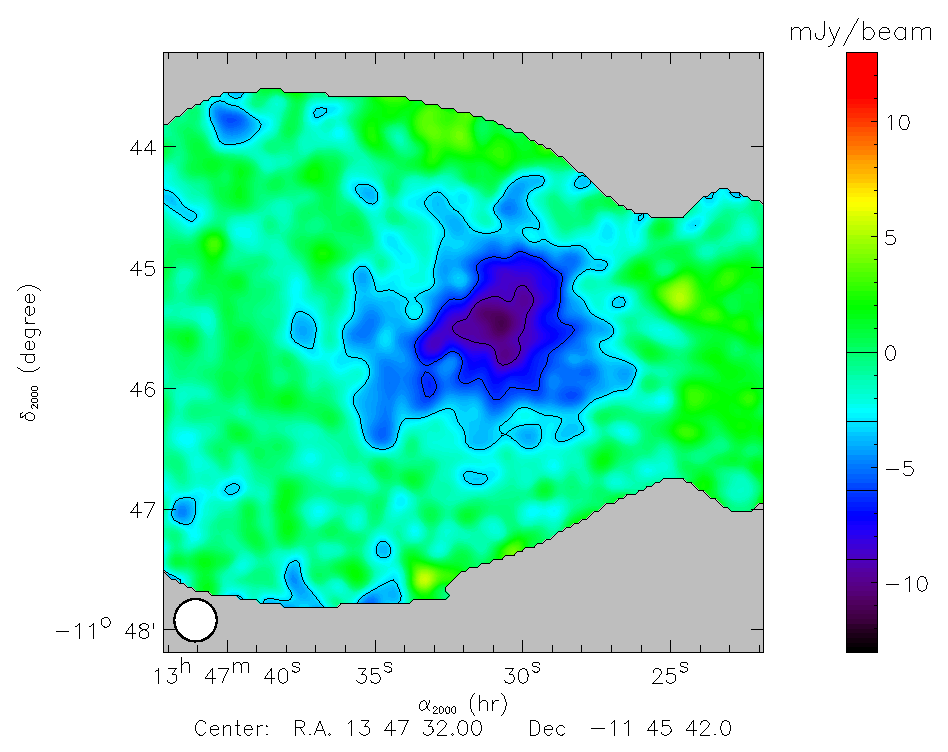
\includegraphics[width=0.32\textwidth]{./RXJ1347-1145_PS_subtracted_map_2mm.eps}
	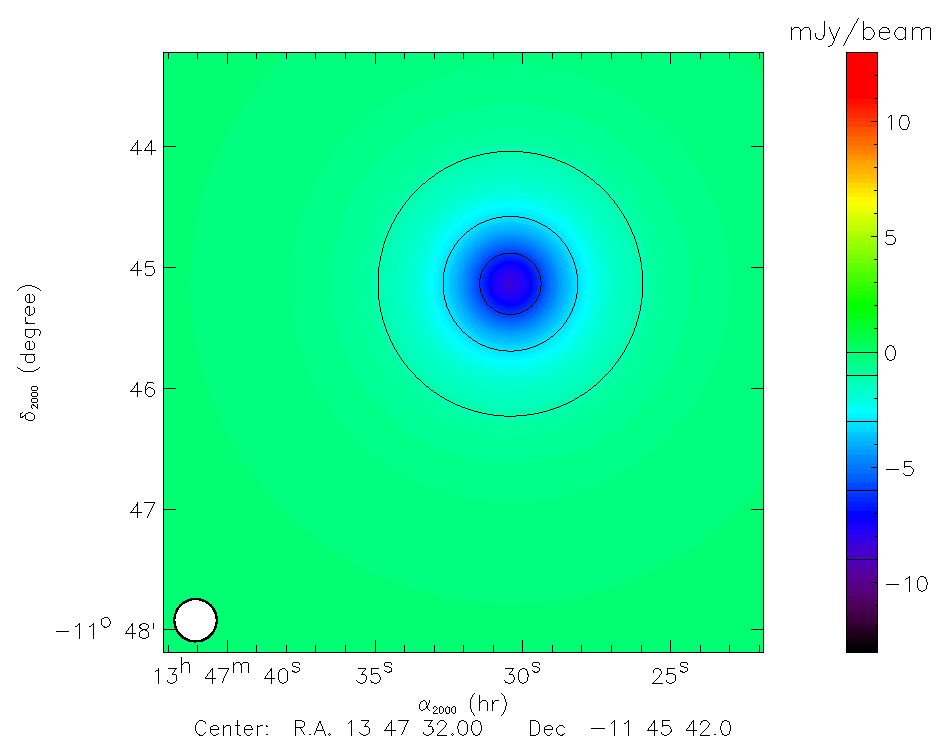
\includegraphics[width=0.32\textwidth]{./model.eps}
	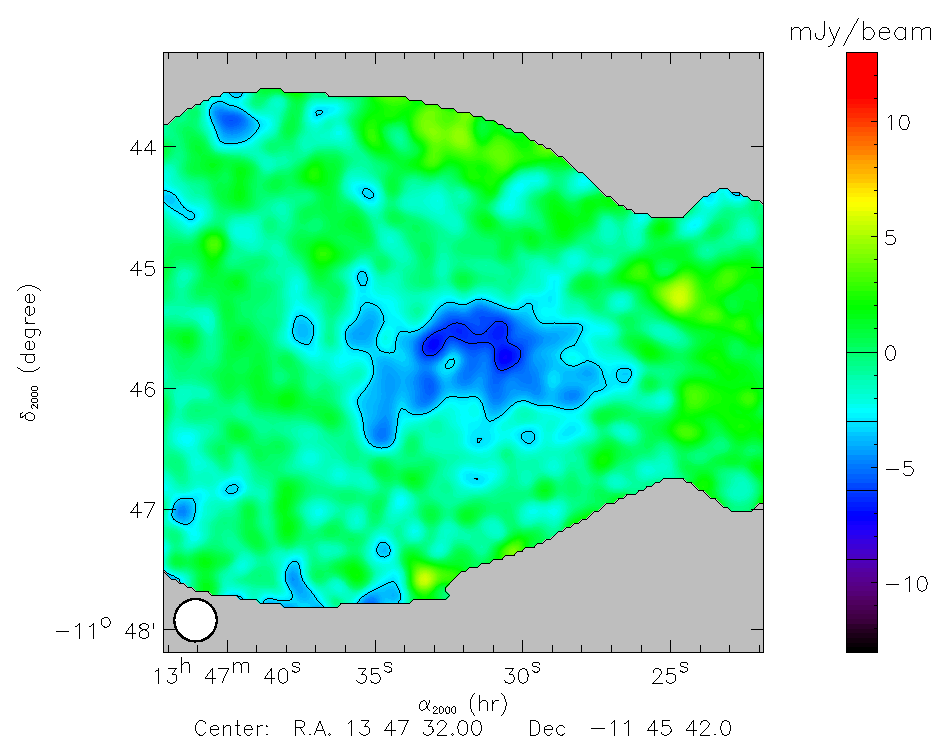
\includegraphics[width=0.32\textwidth]{./residu.eps}
	\caption{Comparison between the original radio point source subtracted map of RX~J1347.5-1145 (left) and the relaxed cluster best fit model map excluding the shock area, centered on the X-ray peak (middle). Residuals are given on the right panel. The model accounts well for the cluster profile and agree with X-ray data, except in the southern shocked area that is revealed by the residual map. The SNR of the tSZ peak is about 10 on the left panel map.}
        \label{fig:rxj}
	
	\centering
	\includegraphics[width=0.5\textwidth]{./cluster_profiles.eps}
	\caption{Estimated absolute value of the flux density profiles of the selected galaxy clusters as derived from X-ray data \citep{Barbara}, at 140 GHz. This is a lower limit estimate of the signal since it does not account for overpressure caused by shocks at the substructure level, that are well seen in tSZ and reinforce the signal. For instance, the substructures present in the NIKA map of MACS~J0717.5+3745 (Fig.~\ref{fig:macsj0717}) reach up to $\sim$ 5 mJy/Beam while the profile would suggest a tSZ peak of $\sim$ 3 mJy/Beam. Since the MUSTANG map of CL 1226.9+3332 reveals strong disturbed tSZ signal, we can also safely expect a signal stronger than indicated by the profile, up to 6-7 mJy/beam at the scales recovered by MUSTANG, $\sim$~60~arcsec. RX~J1347.5-1145 is included as a reference since it has already been observed.}
        \label{fig:exp_prof}

	%%%%%%%%%% Table %%%%%%%%�
	\begin{center}
	\begin{tabular}{|p{3.5cm}|p{2cm}|p{1.5cm}|p{8.5cm}|}
	\hline
	Cluster & $\theta_{\mathrm{s}}$ (arcsec) & $z$ & Comment \\
	\hline
	MACS~J0717.5+3745 & 109 & 0.55 & Triple-merger, 2 strong tSZ substructures at $\sim$ 30".\\
	CL~1226.9+3332 & 67 & 0.89 & Disturbed in X-ray. Compact.\\
	MACS~J1423.8+2404 & 76 & 0.54 &  Spherically symmetric and relaxed. Faint central radio source ($\sim$ 0.1 mJy at 140 GHz).\\
	RX~J1347.5-1145 & 70 & 0.45 & Strong south-east tSZ extension (shock). Central radio source ($\sim$ 4 mJy at 140 GHz).\\
	\hline
	\end{tabular}
	\end{center}
	\caption{Main characteristics of the target clusters based on X-ray, optical and other tSZ data. RX~J1347.5-1145 is included as a reference since it has already been observed.}
	\label{tab:list_gc}
	\end{figure}
	
	\begin{figure}[t]
	\centering	
	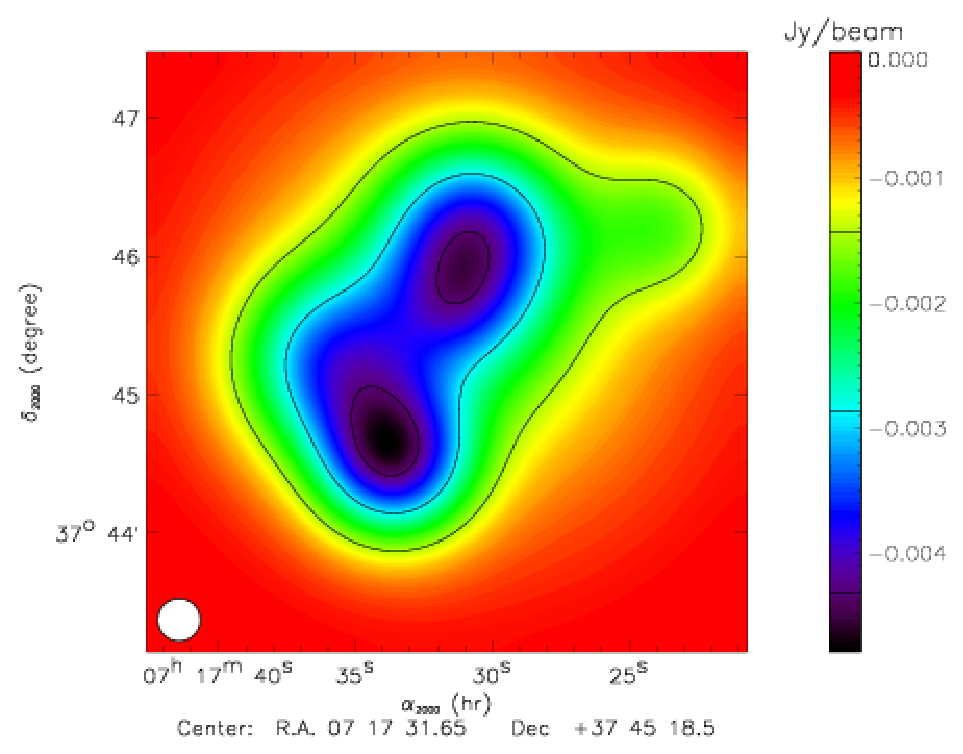
\includegraphics[width=0.37\textwidth, trim=0cm -2.7cm 0cm 0cm, clip=true]{./MACSJ0717_model.eps}
	\hspace*{1cm}
	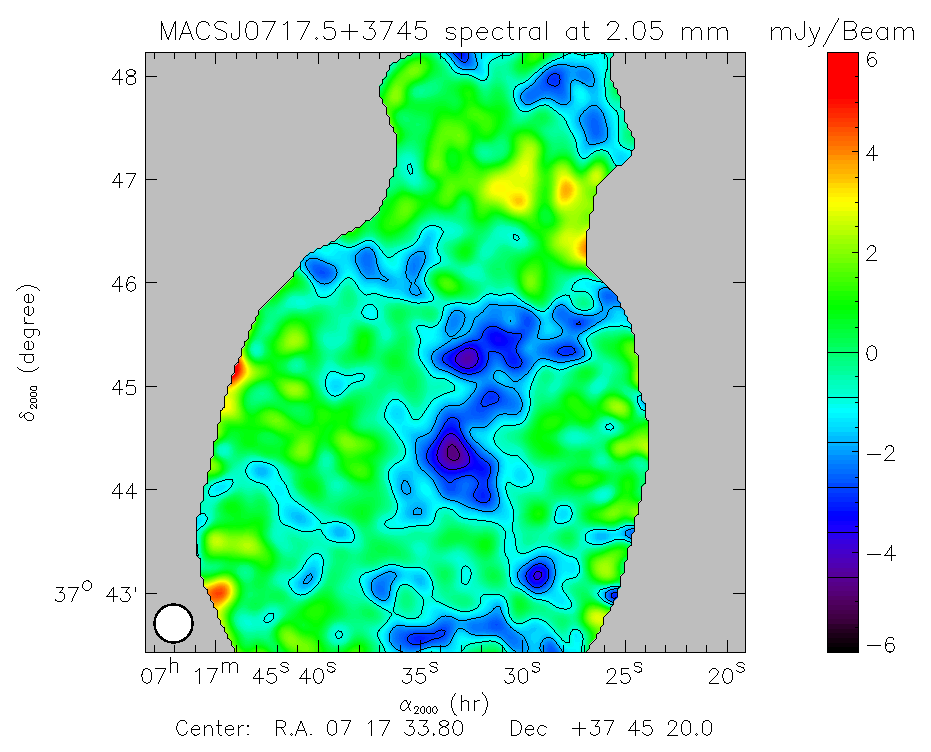
\includegraphics[width=0.5\textwidth]{./MACSJ0717_NIKA.eps}
	\caption{Left: estimation of the tSZ map of MACS J0717.5+3745 based on X-ray and optical data, at 140 GHz. Right: NIKA 140 GHz map obtained during Run5 test observations. This map already shows the presence of two main substructures. The north one corresponds to the high density X-ray core of the cluster, where an optical sub cluster is detected. The southern clump is related to the merging of two other optically detected groups. This tSZ map indicates that the ICM temperature at play is extremely high particularly in the southern clump (maybe higher than 25 keV). The tSZ peaks reach a SNR of 5, giving precious informations for future observations but not sufficient for a detailed study.}
        \label{fig:macsj0717}
	\end{figure}
	

% Bibliography and bibfile
\def\aj{AJ}%
          % Astronomical Journal
\def\actaa{Acta Astron.}%
          % Acta Astronomica
\def\araa{ARA\&A}%
          % Annual Review of Astron and Astrophys
\def\apj{ApJ}%
          % Astrophysical Journal
\def\apjl{ApJ}%
          % Astrophysical Journal, Letters
\def\apjs{ApJS}%
          % Astrophysical Journal, Supplement
\def\ao{Appl.~Opt.}%
          % Applied Optics
\def\apss{Ap\&SS}%
          % Astrophysics and Space Science
\def\aap{A\&A}%
          % Astronomy and Astrophysics
\def\aapr{A\&A~Rev.}%
          % Astronomy and Astrophysics Reviews
\def\aaps{A\&AS}%
          % Astronomy and Astrophysics, Supplement
\def\azh{AZh}%
          % Astronomicheskii Zhurnal
\def\baas{BAAS}%
          % Bulletin of the AAS
\def\bac{Bull. astr. Inst. Czechosl.}%
          % Bulletin of the Astronomical Institutes of Czechoslovakia 
\def\caa{Chinese Astron. Astrophys.}%
          % Chinese Astronomy and Astrophysics
\def\cjaa{Chinese J. Astron. Astrophys.}%
          % Chinese Journal of Astronomy and Astrophysics
\def\icarus{Icarus}%
          % Icarus
\def\jcap{J. Cosmology Astropart. Phys.}%
          % Journal of Cosmology and Astroparticle Physics
\def\jrasc{JRASC}%
          % Journal of the RAS of Canada
\def\mnras{MNRAS}%
          % Monthly Notices of the RAS
\def\memras{MmRAS}%
          % Memoirs of the RAS
\def\na{New A}%
          % New Astronomy
\def\nar{New A Rev.}%
          % New Astronomy Review
\def\pasa{PASA}%
          % Publications of the Astron. Soc. of Australia
\def\pra{Phys.~Rev.~A}%
          % Physical Review A: General Physics
\def\prb{Phys.~Rev.~B}%
          % Physical Review B: Solid State
\def\prc{Phys.~Rev.~C}%
          % Physical Review C
\def\prd{Phys.~Rev.~D}%
          % Physical Review D
\def\pre{Phys.~Rev.~E}%
          % Physical Review E
\def\prl{Phys.~Rev.~Lett.}%
          % Physical Review Letters
\def\pasp{PASP}%
          % Publications of the ASP
\def\pasj{PASJ}%
          % Publications of the ASJ
\def\qjras{QJRAS}%
          % Quarterly Journal of the RAS
\def\rmxaa{Rev. Mexicana Astron. Astrofis.}%
          % Revista Mexicana de Astronomia y Astrofisica
\def\skytel{S\&T}%
          % Sky and Telescope
\def\solphys{Sol.~Phys.}%
          % Solar Physics
\def\sovast{Soviet~Ast.}%
          % Soviet Astronomy
\def\ssr{Space~Sci.~Rev.}%
          % Space Science Reviews
\def\zap{ZAp}%
          % Zeitschrift fuer Astrophysik
\def\nat{Nature}%
          % Nature
\def\iaucirc{IAU~Circ.}%
          % IAU Cirulars
\def\aplett{Astrophys.~Lett.}%
          % Astrophysics Letters
\def\apspr{Astrophys.~Space~Phys.~Res.}%
          % Astrophysics Space Physics Research
\def\bain{Bull.~Astron.~Inst.~Netherlands}%
          % Bulletin Astronomical Institute of the Netherlands
\def\fcp{Fund.~Cosmic~Phys.}%
          % Fundamental Cosmic Physics
\def\gca{Geochim.~Cosmochim.~Acta}%
          % Geochimica Cosmochimica Acta
\def\grl{Geophys.~Res.~Lett.}%
          % Geophysics Research Letters
\def\jcp{J.~Chem.~Phys.}%
          % Journal of Chemical Physics
\def\jgr{J.~Geophys.~Res.}%
          % Journal of Geophysics Research
\def\jqsrt{J.~Quant.~Spec.~Radiat.~Transf.}%
          % Journal of Quantitiative Spectroscopy and Radiative Trasfer
\def\memsai{Mem.~Soc.~Astron.~Italiana}%
          % Mem. Societa Astronomica Italiana
\def\nphysa{Nucl.~Phys.~A}%
          % Nuclear Physics A
\def\physrep{Phys.~Rep.}%
          % Physics Reports
\def\physscr{Phys.~Scr}%
          % Physica Scripta
\def\planss{Planet.~Space~Sci.}%
          % Planetary Space Science
\def\procspie{Proc.~SPIE}%
          % Proceedings of the SPIE
\let\astap=\aap
\let\apjlett=\apjl
\let\apjsupp=\apjs
\let\applopt=\ao
%
	

\bibliography{biblio}

%----------------------------------------------------------------
% Extended Source List (sources which do not fit on cover page)
%  -  place anywhere after the cover page  
%  -  uncomment the following 5 lines if needed
%  -  do NOT modify the format
%----------------------------------------------------------------
% \extendedsourcelist{
% L1448       & 03:25:38.9   & +30:44:05       & +5.0  \\
% M33         & 01:33:50.9   & +30:39:35.8     & -170  \\
% ...         &  ...         &    ....         &  ...  \\
% }
%----------------------------------------------------------------

\end{document}
